\documentclass{article}
\usepackage{graphicx} % Required for inserting images
\usepackage[top=0.9in, bottom=1in, left=1.5in, right=1.5in]{geometry}
\usepackage[utf8]{inputenc}
\usepackage[icelandic]{babel}
\usepackage[T1]{fontenc}
\usepackage[sc]{mathpazo}
\usepackage[parfill]{parskip}
\renewcommand{\baselinestretch}{1.2}
\usepackage{booktabs,tabularx}
\usepackage{multirow}
\usepackage{enumerate}
\usepackage{adjustbox}
\usepackage{multicol}
\usepackage{xcolor}
\usepackage{algpseudocode}
\usepackage{tikz}
\usepackage{nicefrac}
\usepackage{changepage}
\usetikzlibrary{arrows, positioning, calc, graphs}
\usepackage{amsmath, amsfonts, amssymb, amsthm}
\usepackage{graphicx}
\usepackage{tikz}
\usepackage{minted}
\usemintedstyle{manni}
\title{Forritunarmál Hópverkefni 9}
\author{Ragnar Björn Ingvarsson, rbi3 \\
		Daníel Snær Halldórsson, dsh11 \\
		Ólafur Sær Sigursteinsson, oss27}
\tikzset{->, >=stealth', shorten >=1pt, node distance=2cm,thick, main node/.style={circle,draw,minimum size=3em}}

\begin{document}
\renewcommand\thepage{}

	\maketitle

	\newpage
	\begin{verbatim}
;;;;;;;;;;;;;;;;;;;;;;;;;;;;;;;;;;;;;;;;;;;;
;;;
;;; Design document
;;; ===============
;;;
;;; Exported
;;; --------
;;;
;;; Use:   val s = makeSet();
;;; Pre:   Nothing.
;;; Post:  s contains a new empty set of
;;;        values that are allowed as
;;;        arguments to the imported
;;;        function comp.
;;;
;;; Imported
;;; --------
;;;
;;; Use:  val c = comp(x,y);
;;; Pre:  x and y are values that are 
;;;       allowed to be stored in the sets
;;;       implemented here.
;;; Post: c is an integer that is <0 if x
;;;       must precede y, >0 if y must
;;;       precede x, and ==0 if x and y
;;;       are equal.
;;; Note: comp should define an ordering on
;;;       the values allowed in the sets.
;;;       The ordering should ensure that
;;;       any finite set of values has a
;;;       least element.
;;;
;;; Use:  s.add(x);
;;; Pre:  s is a set that can contain x.
;;; Post: x has been added to s if it was
;;;       not already in s. If x was
;;;       was already in s then s is
;;;       unchanged.
;;;
;;; Use:  val e = s.isEmpty();
;;; Pre:  s is a set.
;;; Post: e contains true if s is empty,
;;;       false otherwise.
;;;
;;; Use:  val c = s.contains(x);
;;; Pre:  s is a set that can contain x.
;;; Post: c is true if s contains x, false
;;;       otherwise.
;;;
;;; Use:  val m = s.min();
;;; Pre:  s is a set, not empty.
;;; Post: m is the minimal value in s,
;;;       according to the imported
;;;       function comp.
;;;
;;; Use:  s.remove(x);
;;; Pre:  s is a set that can contain x.
;;; Post: If s contained x then x has
;;;       been removed from s, otherwise
;;;       s is unchanged.
;;;
;;; Use:  val r = s.mapReduce(op,f,u);
;;; Pre:  s is a set.
;;;       op is a binary function,
;;;       f is a unary function.
;;;       u is some value such that
;;;       the expression in the post-
;;;       condition can be computed.
;;; Post: The expression
;;;        u ! f(x1) ! f(x2) ! ... ! f(xN)
;;;       has been computed, where x!y
;;;       is equivalent to op(x,y) and
;;;       the computation is performed
;;;       from left to right, and the
;;;       values x1,x2,...,xN are all the
;;;       values in s in ascending order.
;;;
;;;;;;;;;;;;;;;;;;;;;;;;;;;;;;;;;;;;;;;;;;;;

"set.mmod" =
{{
makeSet = fun makeSet();
}}
*
!
{{
makeSet =
    obj()
    {
    
        var set = [];
        
        ;;; Data invariant:
        ;;;   A set of values allowed as arguments to the
        ;;;   imported function comp, where each element only
        ;;;   appears once, represented as an ordered tree 
        ;;;   according to the imported module orderedtree.
        
        msg add(x)
        {
            set = insert(set,x);
        };
        
        msg isEmpty()
        {
            if ( set == [] ) { return true };
            return false;
        };
        
        msg contains(x)
        {
            return contains(set,x);
        };
        
        msg min()
        {
            return min(set);
        };
        
        msg remove(x)
        {
            set = remove(set,x);
        };
        
        msg mapReduce(op,f,u)
        {
            ;;; Use:  z = help(x,op,f,u)
            ;;; Pre:  x is an ordered tree of values 
            ;;;       allowed as arguments to f.
            ;;;       op is a binary function, f is a unary
            ;;;       function and u is a value such that the value
            ;;;       in the post-condition can be evaluated.
            ;;; Post: z contains the value of the expression 
            ;;;       u ! f(x1) ! f(x2) ! ... ! f(xN)
            ;;;       where x!y is equivalent to op(x,y) and
            ;;;       the computation is performed
            ;;;       from left to right and x1 is the minimum
            ;;;       value in the tree and xN is the maximum.
            rec fun help(x, op, f, u)
            {
                if ( x == [] )
                {
                    return u;
                };
                return help( remove(x,min(x)), op, f, op(u, f(min(x))));
            };
            return help(set, op, f, u);
        };
    };
}}
*
"orderedtree.mmod"
;
	\end{verbatim}
	\begin{center}
		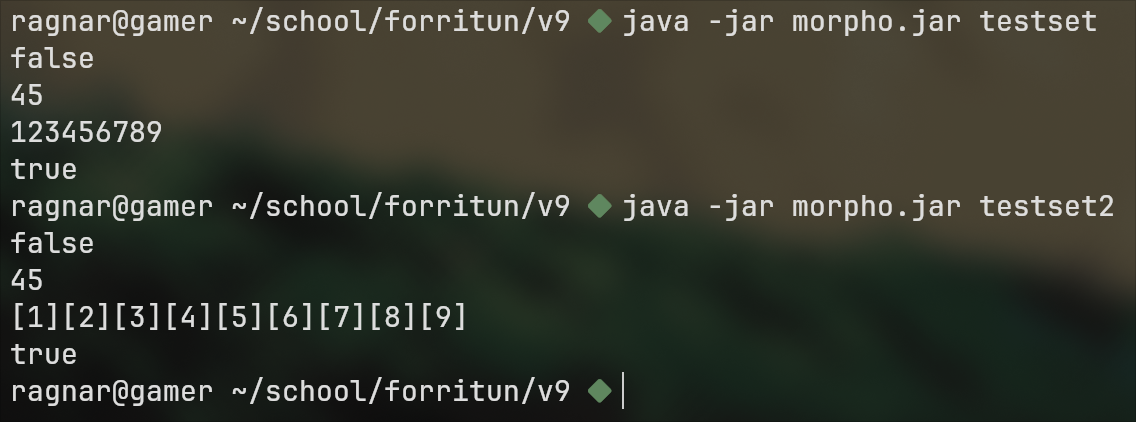
\includegraphics[scale=0.33]{set.png}
	\end{center}
	
\end{document}
